\documentclass[10pt]{article} % For LaTeX2e
%\usepackage{tmlr}
% If accepted, instead use the following line for the camera-ready submission:
%\usepackage[accepted]{tmlr}
% To de-anonymize and remove mentions to TMLR (for example for posting to preprint servers), instead use the following:
\usepackage[preprint]{tmlr}

% Optional math commands from https://github.com/goodfeli/dlbook_notation.
\input{math_commands.tex}

\usepackage{hyperref}
\usepackage{url}
\usepackage{graphicx}
\usepackage{float} 


\title{Reproducing TTP for Safer Pretraining: A Study of Harmful Content Benchmarks}

% Authors must not appear in the submitted version. They should be hidden
% as long as the tmlr package is used without the [accepted] or [preprint] options.
% Non-anonymous submissions will be rejected without review.

\author{\name Ali Bilge \email ali.bilge@student.uva.nl \\
      \addr Faculty of Science\\
      University of Amsterdam
      \AND
      \name Ark Deliev \email ark.deliev@student.uva.nl \\
      \addr Faculty of Science\\
      University of Amsterdam
      \AND
      \name Miguel Mendes \email miguel.aldea.mendes@student.uva.nl\\
      \addr Faculty of Science\\
      University of Amsterdam}

% The \author macro works with any number of authors. Use \AND 
% to separate the names and addresses of multiple authors.

\newcommand{\fix}{\marginpar{FIX}}
\newcommand{\new}{\marginpar{NEW}}

\newcommand{\origTable}[1]{Original Table~#1}
\newcommand{\origFig}[1]{Original Figure~#1}

\def\month{01}  % Insert correct month for camera-ready version
\def\year{2026} % Insert correct year for camera-ready version
\def\openreview{\url{https://openreview.net/forum?id=XXXX}} % Insert correct link to OpenReview for camera-ready version


\begin{document}


\maketitle

\begin{abstract}
We present a reproducibility study of ``Towards Safer Pretraining: Analyzing and Filtering Harmful Content in Webscale Datasets for Responsible LLMs'' (IJCAI 2025). We evaluate four core claims using released artifacts, focusing on the TTP prompt-based classifier, the HarmFormer model, and the HAVOC benchmark. Our reproduction yields mixed results: HAVOC leakage is reproduced, while TTP performance on TTP-Eval and OpenAI Moderation deviates from the original claims. HarmFormer generalizes reasonably to human-annotated data, and cross-model tests show partial portability but strong sensitivity to output formatting, especially for open-source backbones. We summarize these findings and discuss implications for reproducibility and deployment.
\end{abstract}

\section{Introduction}

Large language models (LLMs) are increasingly pretrained on massive web-scale datasets, raising growing concerns about the presence of harmful, toxic, or manipulative content in their training data \citep{bender2021stochasticparrots}. Prior work has shown that large web corpora often lack sufficient documentation and transparency, making it difficult to assess data quality and potential risks introduced during pretraining \citep{dodge2021c4}. Moreover, evaluating and mitigating harmful content frequently relies on automatic or model-based judgments, which are known to be imperfect and sensitive to evaluation design choices \citep{welbl2021detoxchallenges}. Since pretraining data directly shapes downstream model behavior, understanding and mitigating harmful content has become a central issue in responsible AI development.

The IJCAI 2025 paper \textit{Towards Safer Pretraining: Analyzing and Filtering Harmful Content in Webscale Datasets for Responsible LLMs} addresses this challenge by proposing a taxonomy-driven framework for analyzing harmful content in web data and by introducing tools to support safer pretraining \citep{mendu2025saferpretraining}. The authors define a structured taxonomy that distinguishes between safe, topical, and toxic content, building on earlier efforts to study toxic language in language model outputs and training data \citep{gehman2020realtoxicityprompts}. In addition, the paper introduces several resources, including the TTP benchmark for prompt-based harmful content identification, the HAVOC benchmark for adversarial prompt evaluation, and the HarmFormer model for long-form harmful content classification. These contributions align with a broader line of work on adversarial prompting and robustness benchmarking.

In this work, we examine the reproducibility of the results reported in the original paper. While the authors make several components publicly available, such as prompt templates and benchmark datasets, some aspects of the large-scale data processing and filtering pipeline are described at a high level. We aim to follow the methodology as closely as possible and, where necessary, reimplement missing components based on the descriptions provided in the paper and accompanying resources.

Our reproduction therefore investigates both the extent to which the reported results can be recovered using the released artifacts and the feasibility of reconstructing additional parts of the pipeline in practice.

\section{Related Work}

Prior work related to this study spans research on web-scale dataset transparency, harmful content detection tools, and toxicity evaluation benchmarks.

\subsection{Web-Scale Data and Transparency}

Web-scale datasets are widely used for pretraining language models, but their opacity raises concerns about data quality, bias, and downstream harms. \citet{dodge2021c4} document limitations in dataset transparency for corpora such as C4, motivating clearer reporting of data curation practices. \citet{luccioni2021whatsinthebox} analyze undesirable content in Common Crawl using keyword heuristics, while \citet{jansen2022perplexity} propose perplexity-based filtering to remove toxic text. However, these methods lack precision: keyword filters can conflate harmful intent with educational content, and perplexity thresholds fail to capture contextual nuances.

\subsection{Content Moderation Tools}

Existing approaches to harmful content detection rely on keyword blocklists (such as the LDNOOBW list\footnote{\url{https://github.com/LDNOOBW/List-of-Dirty-Naughty-Obscene-and-Otherwise-Bad-Words}}) and API-based tools. Perspective API\footnote{\url{https://perspectiveapi.com/}} is widely used for toxicity detection but suffers from critical limitations: it is designed for sentence-level analysis and uses binary taxonomies that conflate harmful intent with socially critical discourse \citep{mendu2025saferpretraining}. Model-based approaches include HateBERT \citep{caselli2021hatebert}, a BERT-based model fine-tuned on hate speech datasets, and Llama Guard \citep{inan2023llamaguard}, an LLM-based input-output safeguard for conversational AI. The original authors demonstrate that these tools exhibit poor generalization across harm categories and struggle with long-form content, motivating their three-dimensional taxonomy (Safe, Topical, Toxic) and multi-harm coverage.

\subsection{Toxicity Evaluation Benchmarks}

RealToxicityPrompts (RTP) \citep{gehman2020realtoxicityprompts} evaluates toxic degeneration in language model outputs using 100K prompts scored by Perspective API. However, RTP focuses narrowly on toxicity and sexual content, and subsequent work shows that automatic toxicity assessment is sensitive to model choice and evaluation design \citep{welbl2021detoxchallenges}. To address these limitations, the original authors introduce HAVOC (Harmful Abstractions and Violations in Open Completions), a multidimensional benchmark with 10,376 adversarial prompts spanning five harm categories. Unlike RTP, HAVOC distinguishes between neutral, passive (topical), and provocative inputs, revealing that state-of-the-art LLMs exhibit harmful content in 26.7\% of outputs.

\subsection{Contributions of the Original Work}

The work of \citet{mendu2025saferpretraining} integrates structured taxonomies with prompt-based (TTP) and model-based (HarmFormer) tools for large-scale harmful content analysis. Our study focuses on assessing the reproducibility of these contributions using the publicly released artifacts, including the TTP prompt templates, HAVOC benchmark, TTP-Eval evaluation set, and the HarmFormer model weights.


\section{Scope of Reproducibility}

We focus on reproducing the core claims regarding the performance and effectiveness of the TTP prompt and HarmFormer model, as well as validating the HAVOC benchmark results. Specifically, we aim to verify the following claims from the original work:

We verify four claims from \citet{mendu2025saferpretraining}:
\textbf{Claim 1 (TTP Performance)}: 0.87 precision, 0.79 recall, 0.83 F1 on TTP-Eval (\origTable{3});
\textbf{Claim 2 (HarmFormer Performance)}: 0.88 precision, 0.81 recall, 0.85 F1 on the authors' internal split (\origTable{6}), noting we instead evaluate on TTP-Eval;
\textbf{Claim 3 (Baseline Comparison)}: TTP and HarmFormer outperform baselines on OpenAI Moderation (\origTable{7}), evaluated here against Perspective and Llama Guard with TTP via OpenRouter (gpt-4o);
and \textbf{Claim 4 (HAVOC Leakage)}: 26.7\% overall leakage with 76\% on provocative inputs (\origTable{10}, \origFig{3}), computed from released \texttt{havoc\_modeleval.tsv} generations.


All results in this paper are generated from our reproduction code (anonymized: \url{https://anonymous.4open.science/r/TowardsSaferPretraining-6046}).

\paragraph{Communication with original authors.}
We contacted the original authors during the project to request clarifications and missing artifacts needed for strict comparability (e.g., the internal HarmFormer test split and evaluation details). We did not receive a response by the submission deadline. Therefore, all results reported in this paper rely solely on publicly released artifacts and documentation.

Due to computational and budgetary constraints, we do not reproduce the large-scale dataset annotation pipeline described in Section 5.1 of the original paper, which involves labeling 3 million web pages. We also do not reproduce the model architecture comparison experiments (\origTable{5}), as we use the pre-trained HarmFormer model released by the authors rather than training from scratch.


We focus our experimental validation on reproducing \origTable{3}, \origTable{4}, \origTable{6}, \origTable{7}, and \origTable{10}, and \origFig{3} from the original paper.
 We do not attempt to reproduce \origTable{5} (model architecture comparison requiring retraining), \origTable{8} (3M sample dataset analysis), \origFig{2} (domain distribution), or \origFig{5}. \origTable{1}, \origTable{2}, and \origTable{9} are definitional or descriptive and do not require experimental reproduction. Our code produces the reproduced tables and \origFig{3} using the released artifacts; other figures are added to explain our extensions.
Our reproduction therefore focuses on validating the effectiveness of the released artifacts for harmful content detection, rather than reconstructing the full data curation and model training pipeline.


\section{Methodology}

\subsection{Model Descriptions}

\textbf{TTP (Topical \& Toxic Prompt)}
TTP is a prompt-based classifier built on OpenAI's GPT-4 Omni (gpt-4o) via an OpenAI-compatible API endpoint (OpenRouter in our runs). The prompt implements the three-dimensional taxonomy (Safe, Topical, Toxic) across five harm categories: Hate \& Violence, Ideological Harm, Sexual Content, Illegal Activities, and Self-Inflicted Harm. We use the exact prompt templates released in the authors' GitHub repository\footnote{\url{https://github.com/themendu/TowardsSaferPretraining}} with greedy decoding (temperature = 0) to maximize reproducibility.
The original paper notes that the TTP prompt was iteratively tuned on a held-out development set using few-shot and chain-of-thought prompting with GPT-4-Omni; we therefore use the released prompt and retain its reasoning and label format. A remaining source of discrepancy is the API endpoint: the paper uses OpenAI's GPT-4-Omni directly, while our runs use GPT-4o via OpenRouter. For API-backed TTP runs we do not apply explicit truncation; for local TTP runs we cap the input length (default 8{,}192 tokens) to reduce KV-cache memory usage.

\textbf{HarmFormer}
HarmFormer is a fine-tuned LongFormer-based model \citep{beltagy2020longformer} with 1024-token context length. The model employs a multi-task architecture with five classification heads corresponding to the harm categories, where each head classifies content into Safe, Topical, or Toxic dimensions. We use the pre-trained model weights released on HuggingFace\footnote{\url{https://huggingface.co/themendu/HarmFormer}} and define a document as Toxic if any head predicts Toxic.

\subsection{Datasets}

We evaluate our reproduction on three datasets used in the original paper:

\textbf{TTP-Eval} consists of 393 expert-annotated web pages spanning all five harm categories, with content labeled across the three-dimensional taxonomy (Safe, Topical, Toxic). The dataset exhibits high inter-annotator agreement (Krippendorff's Alpha = 0.77) and includes documents of varying lengths. We use this benchmark to validate Claim 1 (TTP performance). For Claim 2, we also evaluate HarmFormer on TTP-Eval, though this differs from the original \origTable{6} evaluation which uses the authors' internal test split from the 253K TTP-labeled dataset (90:5:5 train/dev/test split). Our HarmFormer evaluation therefore assesses generalization to human-annotated data rather than exact reproduction of \origTable{6}.

\textbf{HAVOC} (Harmful Abstractions and Violations in Open Completions) contains 10,376 adversarial prompt snippets designed to evaluate LLM safety across five harm categories. The benchmark distinguishes three input types: Neutral (seemingly benign prompts), Passive (topical discussion prompts), and Provocative (explicitly harmful prompts). In the original paper six open-source models are evaluated: Gemma 2 (2B, 9B, 27B), Llama 3.2 (1B, 3B), and Mistral 7B v0.3. For HAVOC evaluation, we use the pre-computed model generations released by the authors in \texttt{havoc\_modeleval.tsv}. This file contains prefix-suffix pairs with model responses and TTP-based judge annotations already computed for all six models. We compute leakage metrics directly from these annotations without running model inference, which matches \origTable{10}  of the original paper.

\textbf{OpenAI Moderation test set} \citep{markov2023openai} contains 1,680 sentences (1,158 non-toxic, 522 toxic) across four categories: Sexual, Hate, Violence, and Self-Harm. Following the original paper's approach, we aggregate these categories into a single binary label (Toxic vs. Non-Toxic) for evaluation. We compare TTP and HarmFormer against Perspective (max toxicity over 500-character chunks, threshold 0.4) and Llama Guard 3 (focused, zero-shot, few-shot prompts; greedy decoding).
\textbf{Data access and format.}
TTP-Eval is publicly released by the original authors as a tabular dataset (TSV) containing full web-page text, harm category labels, and Safe/Topical/Toxic annotations per category. We use the official release without modification.
\textbf{Label aggregation.}
For overall toxic detection, we assign a document-level Toxic label if any harm category is annotated as Toxic. Otherwise, documents are labeled as Non-Toxic (Safe or Topical), matching the evaluation protocol in the original paper.

 \textbf{The HAVOC dataset} contains 10,376 web-derived prefix–suffix pairs sampled from Common Crawl, C4, and FineWeb. Prefixes have an average length of 26 tokens (minimum: 1, maximum: 891), computed using whitespace tokenization. Each prefix is annotated across five harm dimensions: Hate \& Violence, Ideological Harm, Sexual, Illegal Activities, and Self-Inflicted harm, where labels indicate topical intent rather than explicit toxicity. Approximately 17.9\% of prefixes contain at least one topical harm category, with Hate \& Violence being the most frequent (7.3\%). Multiple harm categories may co-occur within a single prefix.
In our processing, the released \texttt{havoc.tsv} contains a small number of rows with malformed quotation marks; using Python's default CSV parsing can merge lines and reduce the effective sample count. We therefore parse \texttt{havoc.tsv} line-by-line using tab delimiters to ensure all 10,376 rows are loaded.
\textbf{Label Frequency Analysis}. Appendix Figure~\ref{fig:havoc-topical-counts} shows the frequency of topical harm labels in HAVOC. Hate \& Violence appears most often, while Sexual and Illegal labels are less frequent. This highlights the class imbalance in topical content and motivates reporting per-category results.
 \textbf{The TTP-Eval dataset} contains 393 human-annotated web pages with labels across all five harm categories and three severity levels.






%\newpage
\subsection{Hyperparameters}

We follow the original paper: TTP uses greedy decoding (temperature = 0.0, top-p = 1.0); HarmFormer uses the released checkpoint defaults (1024-token context) with no additional fine-tuning; Perspective uses max toxicity over 500-character chunks with threshold 0.4; HAVOC leakage uses the released generations (max 200 output tokens per completion).

\subsection{Experimental Setup and Code}

All experiments are conducted using a combination of cloud API services and academic GPU resources. For TTP evaluation, we use OpenRouter to access GPT-4 Omni (gpt-4o). For HarmFormer inference and for our cross-model extension with Gemma 2 27B, we use an A100 GPU (40GB) provided by our university's academic computing cluster. For HAVOC, unlike the original paper, which uses Ollama as the client-server for running open-source models, we do not run any model ourselves because our Slurm-based cluster environment is not compatible with Ollama, and to avoid unnecessary recomputation. Instead, we use the pre-computed generations and TTP-based annotations provided by the original paper authors to efficiently compute the leakage metrics on CPU.

For API-backed evaluations, we explicitly track parsing/format failures and apply a configurable invalid-output policy (exclude / count-as-non-toxic / count-as-toxic). Unless otherwise stated, the main tables exclude invalid outputs from metric computation; sensitivity analyses can be reproduced using the provided \texttt{--invalid-policy} flag in our scripts.

\subsection{Computational Requirements}

We estimate: TTP on TTP-Eval costs roughly \$5-8 (\~1.5M input and 100K output tokens at GPT-4o pricing); HarmFormer on TTP-Eval takes 1-2 A100 GPU hours; OpenAI Moderation baselines require minimal GPU time plus free but rate-limited Perspective calls; HAVOC leakage uses pre-computed generations and runs in <5 minutes on CPU; and the Gemma 2 27B extension adds 1-2 A100 GPU hours. Total estimated cost is \$5-15, with HAVOC adding no GPU cost.


\section{Results}

\subsection{TTP Performance on TTP-Eval}
We report overall and per-harm toxic detection to show where the prompt is conservative versus missing positives.
\begin{table}[H]
\centering
\begin{tabular}{lccc}
\hline
Harm Category & Precision & Recall & F1 \\
\hline
Hate \& Violence & 0.79 & 0.35 & 0.49 \\
Ideological Harm & 0.75 & 0.17 & 0.28 \\
Sexual & 0.95 & 0.55 & 0.70 \\
Illegal & 0.67 & 0.57 & 0.62 \\
Self-Inflicted & 0.67 & 0.17 & 0.27 \\
\hline
Toxic (Overall) & 0.92 & 0.46 & 0.62 \\
\hline
\end{tabular}
\caption{TTP Quality on TTP-Eval (Toxic Dimension)}
\label{tab:ttp-quality}
\end{table}

Table~\ref{tab:ttp-quality} reports our reproduction of TTP performance on the TTP-Eval benchmark. We observe a precision of 0.92 and recall of 0.46, yielding an F1 score of 0.62 for overall toxic detection. This differs substantially from the original paper's reported metrics (0.87 precision, 0.79 recall, 0.83 F1). While our reproduction achieves higher precision, recall is significantly lower, suggesting the model may be more conservative in its toxic classifications than reported.

Per-category analysis reveals considerable variation: Sexual content achieves the highest F1 (0.70) with 0.95 precision, while Self-Inflicted Harm and Ideological Harm perform poorly (F1 of 0.27 and 0.28 respectively), primarily due to low recall. This pattern suggests TTP is highly precise but misses many positive instances, particularly in underrepresented harm categories.

\subsection{HarmFormer Performance}
We evaluate the model-based classifier on the same benchmark for a direct comparison with TTP.

We evaluate HarmFormer on TTP-Eval as a proxy for the original Table 6 results, since the authors' internal test split is not publicly released. Appendix Table~\ref{tab:harmformer-quality} shows HarmFormer achieves 0.83 precision, 0.74 recall, and 0.78 F1 on overall toxic detection. While not directly comparable to the original claims (0.88 P, 0.81 R, 0.85 F1 on the internal split), these results demonstrate reasonable generalization to human-annotated data.
Notably, HarmFormer outperforms TTP on TTP-Eval (0.78 vs 0.62 F1), primarily due to substantially higher recall (0.74 vs 0.46). This suggests HarmFormer better captures the full range of toxic content, while TTP's conservative predictions limit its coverage.
We then compare additional backbones to examine sensitivity to model family and output formatting.

Appendix Table~\ref{tab:ttp-baselines} compares TTP across different backbone models on TTP-Eval. Our Gemini 2.0 Flash rerun completed with 391 evaluated samples (0.80 F1). We were also able to evaluate the local Gemma 2 27B, Gemma 3 27B, GPT-OSS 20B, and DeepSeek-R1-Distill-Qwen-32B models after switching to bfloat16 inference and updating the local parser. Gemma 2 yields high precision but low recall (0.35 F1), while Gemma 3 improves to 0.57 F1. GPT-OSS 20B reaches 0.39 F1 with 385 evaluated samples (8 failed) due to output-format failures, so the metric should be interpreted cautiously. The R1 distill model attains a stronger balance (0.63 F1). These results reinforce that TTP performance is highly dependent on the underlying model and output formatting, motivating our extension on cross-model generalization.

\subsection{HAVOC Leakage Rates}
Leakage is computed from released generations to avoid re-running models while preserving the original evaluation protocol.
\begin{table}[H]
\centering
\begin{tabular}{lcccc}
\hline
Model & Neutral & Passive & Provocative & Overall \\
\hline
Gemma 2 2B & 9.35 & 12.02 & 76.71 & 26.66 \\
Gemma 2 9B & 9.99 & 11.59 & 77.13 & 27.05 \\
Gemma 2 27B & 10.58 & 12.13 & 76.44 & 27.31 \\
Llama 3.2 1B & 9.38 & 13.48 & 75.40 & 26.61 \\
Llama 3.2 3B & 8.95 & 12.07 & 77.75 & 26.70 \\
Mistral 7B & 9.96 & 13.43 & 72.70 & 26.25 \\
\hline
Average & 9.70 & 12.45 & 76.02 & 26.76 \\
\hline
\end{tabular}
\caption{HAVOC leakage by prompt type (\%) using released generations (six-model average)}
\label{tab:havoc}
\end{table}

Table~\ref{tab:havoc} reports leakage rates on the HAVOC benchmark using pre-computed generations from the released artifacts, averaged across the six models evaluated in the original paper. We observe 26.76\% overall leakage, closely matching the original paper's reported 26.7\%. Leakage varies dramatically by input type: Neutral (9.70\%), Passive (12.45\%), and Provocative (76.02\%). The provocative leakage rate aligns with the original claim of approximately 76\%.
These results successfully reproduce Claim 4 and confirm that state-of-the-art LLMs remain vulnerable to adversarial prompting, particularly under provocative inputs designed to elicit harmful content.

\subsection{RTP vs. HAVOC Leakage (Continuation-Based)}
To mirror the HAVOC vs. RTP comparison in \origFig{3} of the original paper, we compute leakage on RealToxicityPrompts using the dataset-provided continuations and HarmFormer as the judge. Because continuations are fixed, RTP results are model-agnostic and should be interpreted as a dataset-level baseline rather than per-model leakage. Appendix Figure~\ref{fig:havoc-rtp-compare} contrasts RTP against our HAVOC averages. RTP yields 22.26\% overall leakage with 71.33\% on provocative prompts. Note that our RTP bars are not directly comparable to the paper’s figure because the paper evaluates model-generated continuations and uses a different judging pipeline; this can shift the neutral/passive rates upward while reducing the provocative/overall rates relative to HAVOC.

\subsection{Baseline Comparisons}
We report binary toxic detection against API and local baselines on the OpenAI Moderation test set.

Appendix Table~\ref{tab:openai-mod} presents results on the OpenAI Moderation dataset. In our OpenRouter run, TTP achieves 0.80 precision, 0.42 recall, and 0.55 F1, underperforming both HarmFormer (0.64 P, 0.84 R, 0.73 F1) and Perspective API (0.74 P, 0.75 R, 0.74 F1). Llama Guard is competitive, with the focused prompt variant reaching 0.81 F1.
These results differ from the original paper's reported TTP performance (0.72 P, 0.91 R), and show substantially lower recall in our reproduction.
In contrast to the original paper's strong TTP performance on OpenAI Moderation, our reproduction suggests that TTP behavior can vary substantially across runs and evaluation conditions.

\subsection{Summary of Reproducibility Findings}
We summarize each claim with reproduced metrics and a qualitative status label.

\subsubsection{Reproduction Criteria}
We use the following criteria to assign a status label. \textit{Reproduced} indicates our result is within a small tolerance of the original claim while matching the original evaluation protocol as closely as possible: for HAVOC leakage, within 1 percentage point (absolute) on the reported overall and provocative rates; for classification F1, within 0.03 absolute F1. \textit{Partially validated} indicates that key artifacts needed for strict comparability were unavailable (e.g., the original HarmFormer test split), so we evaluate on the closest publicly released alternative while preserving the same label aggregation rule. \textit{Not reproduced} indicates the reproduced metric falls outside these tolerances or required protocol deviations.

Table~\ref{tab:reproducibility-summary} summarizes the reproducibility of each claim. Of the four claims investigated, only Claim 4 (HAVOC leakage) was fully reproduced, with near-exact agreement between our results and the original paper. Claim 2 (HarmFormer) was partially validated on a different test set, showing reasonable generalization. Claims 1 and 3 showed notable discrepancies: TTP achieved higher precision but substantially lower recall than reported, resulting in a 21-point F1 gap on TTP-Eval. These findings suggest that while the released artifacts are functional, TTP performance may be sensitive to factors not fully documented in the original work.

\begin{table}[H]
\centering
\begin{tabular}{llccc}
\hline
Claim & Metric & Original & Reproduced & Status \\
\hline
1: TTP on TTP-Eval & F1 & 0.83 & 0.62 & Not reproduced \\
2: HarmFormer & F1 & 0.85 & 0.78 & Partially validated$^*$ \\
3: TTP on OpenAI Mod & F1 & 0.80 & 0.55 & Not reproduced$^{**}$ \\
4: HAVOC leakage & Overall & 26.7\% & 26.76\% & Reproduced \\
\hline
\multicolumn{5}{l}{\small $^*$Evaluated on TTP-Eval instead of unreleased internal test split.} \\
\multicolumn{5}{l}{\small $^{**}$Our OpenRouter run yields P=0.80, R=0.42, F1=0.55.} \\
\end{tabular}
\caption{Summary of Reproducibility Results}
\label{tab:reproducibility-summary}
\end{table}

\paragraph{Key takeaways.}
\begin{itemize}
    \setlength{\itemsep}{0pt}
    \setlength{\parskip}{0pt}
    \setlength{\topsep}{2pt}
    \setlength{\partopsep}{0pt}
    \item HAVOC leakage reproduces closely when computed from released generations and annotations.
    \item TTP shows high precision but substantially lower recall than reported (Claims 1 and 3 not reproduced).
    \item HarmFormer generalizes reasonably to TTP-Eval, but strict comparability is limited by the unreleased internal split (Claim 2 partially validated).
    \item Cross-model TTP performance is highly sensitive to output formatting and parsing.
    \item Multilingual performance drops substantially and unevenly across languages.
\end{itemize}

\section{Extension: Cross-Model TTP Generalization}

\subsection{Motivation}
In \origTable{4} of the original paper, it is shown that TTP performs strongly with GPT-4 class models but poorly with non-GPT models (R1: 0.06 F1; Gemma 2: 0.35 F1). This lack of generalization raises doubts about the paper's reproducibility and accountability, since if TTP is only effective for a specific model family and not robust to other schemes and models, it raises concerns about accessibility and long-term sustainability (practitioners without API access will not be able to adopt this framework).  

\subsection{Approach}
In this extension we investigate whether the proposed taxonomy and prompting scheme (TTP) can generalize across GPT-4o, Gemini 2.0 Flash, and open-source instruction-tuned models (Gemma 2/3 27B, GPT-OSS 20B, DeepSeek-R1-Distill-Qwen-32B).
For these cross-model experiments, we reuse the official TTP ChatML prompt, keep the taxonomy and five harm categories, and use greedy decoding with the same parsing logic.
Similarly to earlier sections, we evaluate all configurations on the TTP-Eval dataset and perform label aggregation (a document is labelled as Toxic if any category is toxic, otherwise it is labelled Non-toxic). 

\subsection{Results}

For each model, the precision, recall and F1 for the toxic dimension are reported in Appendix Table~\ref{tab:ttp-baselines}. In brief: GPT-4o reaches 0.62 F1; Gemini 2.0 Flash is best at 0.80 F1 (391 samples); DeepSeek-R1-Distill-Qwen-32B reaches 0.63 F1; Gemma 2 27B yields 0.35 F1 while Gemma 3 27B improves to 0.57 F1; GPT-OSS 20B reaches 0.39 F1 with 8 failures.
Furthermore, we observed that the Gemma-based TTP outputs and the expected label format for the TTP parser were consistently different, even though we used the same prompt instructions. This led to almost all Gemma outputs being labelled as Non-Toxic, even for examples that GPT-4o correctly classified as Toxic. This behavior suggests a mismatch between the prompt formatting (tuned specifically for GPT-4 models) and the output format of instruction-tuned models like Gemma. This indicates that the failure is due to format incompatibility and not semantic inability to identify content that is toxic.

\subsection{Analysis}

Our extension reveals a more nuanced picture than the original paper suggests. While Gemma 2 27B struggles with the TTP prompt (0.35 F1) due to output-format mismatches, DeepSeek-R1-Distill-Qwen-32B achieves comparable performance to GPT-4o (0.63 vs 0.62 F1), and Gemini 2.0 Flash outperforms GPT-4o (0.80 vs 0.62 F1). GPT-OSS 20B exhibits high precision but frequent format failures, reducing coverage. This suggests that TTP can generalize to some model families, particularly those with strong instruction-following capabilities. The varying results across models indicate that performance depends heavily on output-format compatibility with the TTP parser rather than semantic understanding of harmful content.

\section{Extension: Multilingual Robustness}

\subsection{Motivation}
The original paper notes multilinguality as future work. We therefore test whether the taxonomy and classifiers remain robust when the same documents are translated into other languages, isolating language effects without changing the underlying harm content.

\subsection{Approach}
We translate TTP-Eval into six languages (Spanish, French, German, Arabic, Hindi, and Chinese) using NLLB-200 3.3B and keep the original labels. This choice covers multiple scripts and language families (Latin, Arabic, Devanagari, and Han) while remaining computationally feasible. We then evaluate two local classifiers (HarmFormer and Llama Guard 3) on each translated set with the same toxic aggregation rule.

\subsection{Results}
Figure~\ref{fig:multilingual-f1} summarizes overall toxic F1 across languages (exact values in Appendix Table~\ref{tab:multilingual}). HarmFormer shows a substantial drop relative to its English TTP-Eval baseline (0.73 F1), and the degradation is uneven across languages. For HarmFormer, Spanish is the strongest (0.40 F1) and French the weakest (0.21 F1). Llama Guard shows its best performance on Hindi (0.47 F1) and the weakest on French (0.15 F1), indicating that multilingual robustness is not uniform across scripts or families.

\begin{figure}[t]
    \centering
    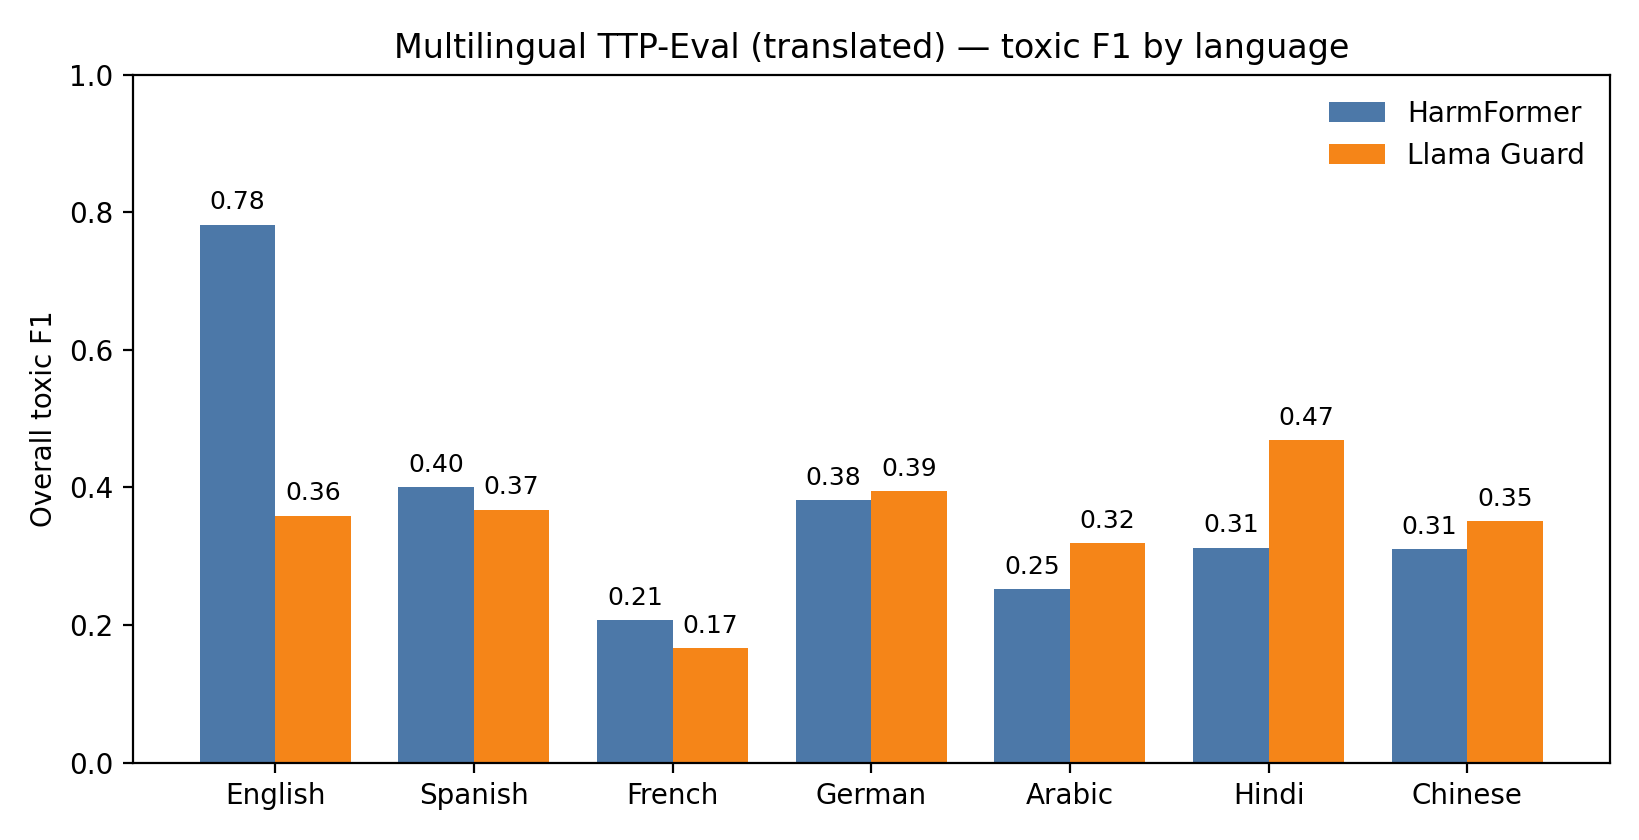
\includegraphics[width=0.85\linewidth]{multilingual-f1.png}
    \caption{Multilingual TTP-Eval toxic F1 by language for HarmFormer and Llama Guard (English shown for reference).}
    \label{fig:multilingual-f1}
\end{figure}

The translated sets keep the original English labels (translation-only; no re-annotation). Machine translation artifacts may influence measured performance.

\subsection{Analysis}
These results suggest that multilingual robustness is a limiting factor even for local classifiers, and that the failure modes vary by language. A key limitation is that we rely on machine translation of TTP-Eval rather than human-verified analogs, so translation artifacts may influence both model behavior and apparent performance. This highlights a practical gap for taxonomy-driven harm detection in non-English settings and motivates prompt adaptation and multilingual training in future work.



\section{Conclusion}

We conducted a reproducibility study of the harmful content detection framework proposed by \citet{mendu2025saferpretraining}. Of the four claims investigated, only the HAVOC leakage results were fully reproduced, with near-exact agreement (26.76\% vs.\ 26.7\%). TTP performance on TTP-Eval showed a substantial gap (0.62 vs.\ 0.83 F1), primarily due to lower recall than reported. HarmFormer demonstrated reasonable generalization to human-annotated data, though direct comparison was limited by the unavailability of the original test split.

Our results highlight two key findings. First, the HAVOC benchmark and pre-computed model generations provide a reliable resource for evaluating LLM safety, with consistent results across our reproduction. Second, while TTP was designed for GPT-4o, our cross-model evaluation shows that some models (Gemini 2.0 Flash, DeepSeek-R1-Distill-Qwen-32B) achieve comparable or better performance, suggesting partial portability. However, output-format compatibility remains a challenge for some model families (e.g., Gemma 2 27B), and GPT-OSS 20B exhibits frequent format failures.

\subsection{Reproducibility Challenges}
Overall, the easiest components to reproduce were those with released artifacts and minimal inference requirements: HAVOC leakage computed from provided generations and HarmFormer inference with published weights. In contrast, API-dependent evaluations (TTP on TTP-Eval and OpenAI Moderation) were harder due to endpoint variance, undocumented prompt/decoding sensitivities, and occasional API failures that affected recall. Local TTP generalization was also challenging: model-family output formats required custom parsing and memory constraints on Snellius necessitated dtype and context-length tuning. These factors explain why artifact-based benchmarks replicated cleanly while prompt- and API-driven results were more fragile.

Future work could investigate the sources of TTP's recall discrepancy, potentially through prompt sensitivity analysis or evaluation on additional datasets. For multilingual evaluation, constructing human-verified analogs of TTP-Eval would reduce translation artifacts and improve interpretability. Developing open-source alternatives to TTP that maintain comparable performance would also increase the accessibility of taxonomy-driven harmful content filtering.

\subsection{Environmental Impact}

%When training and evaluating our models, we tried to avoid the most carbon-intensive parts of the original work so as not incur any unnecessary environmental costs. Instead, we ran our experiments on smaller datasets to save budget and reduce electricity consumption and carbon emissions. Our main compute usage included TTP and HarmFormer on 393 pages (\~1.5M input and 100K output tokens for TTP; 1-2 A100 GPU hours for HarmFormer), OpenAI Moderation evaluation on 1680 sentences, HAVOC leakage computed on CPU from released generations, the Gemma 2 27B extension on an A100, and the multilingual translation/evaluation runs.

%We used CodeCarbon not only to track the energy consumption of our GPU and CPU runs but also to make the costs of reproducibility more transparent. The overall carbon emissions for this project were small compared to training large language models from scratch. Nonetheless, we reduced footprint by reusing released artifacts (e.g., HAVOC generations), limiting model coverage (medium sizes only), and separating local from GPU-intensive jobs to avoid idle allocation.

We minimized environmental costs by reusing released artifacts (e.g., HAVOC generations) and separating local from GPU-intensive jobs to avoid idle allocation. Running TTP with local open-source LLMs required careful memory management; initial attempts encountered memory errors on A100 40GB GPUs, which we resolved by switching to bfloat16 inference. The TTP prompt's extensive taxonomy and few-shot examples require substantial context length, making inference with 27B+ parameter models challenging without precision optimization.

All experiments were conducted on the Snellius HPC cluster (NVIDIA A100-SXM4-40GB, AMD EPYC 7H12 CPUs) and tracked using CodeCarbon. Appendix Table~\ref{tab:compute} summarizes runtime and energy consumption. The total estimated carbon footprint was approximately 0.05 kg CO$_2$, equivalent to driving 0.2 km in an average passenger vehicle. API costs for TTP via OpenRouter totaled \$12.57 USD across 393 requests (\~1.57M tokens).

\subsection{Accountability Implications}

In fields such as machine learning and AI, accountability is a very important concept. It requires that the claims made by researchers be verifiable, that the evaluation procedures be transparent, and that the models' limitations be well documented. These principles are directly connected to our reproducibility study.

Our results reinforce these accountability challenges by identifying which claims can be successfully reproduced, such as the HAVOC leakage analysis, and which cannot, namely, TTP performance and its baseline comparisons. This demonstrates that accountability in AI is more than just releasing code and data, it also involves designing evaluation pipelines that are functional across different models and languages. Without this, even strong-performing claims may not hold up under independent verification.



\newpage
\bibliography{tmlr}
\bibliographystyle{tmlr}

\appendix
\section{Appendix}
\renewcommand{\thetable}{\thesection\arabic{table}}
\renewcommand{\thefigure}{\thesection\arabic{figure}}
\setcounter{table}{0}
\setcounter{figure}{0}

\subsection{Additional Figures and Tables}
\label{sec:appendix-figures}

\begin{figure}[H]
    \centering
    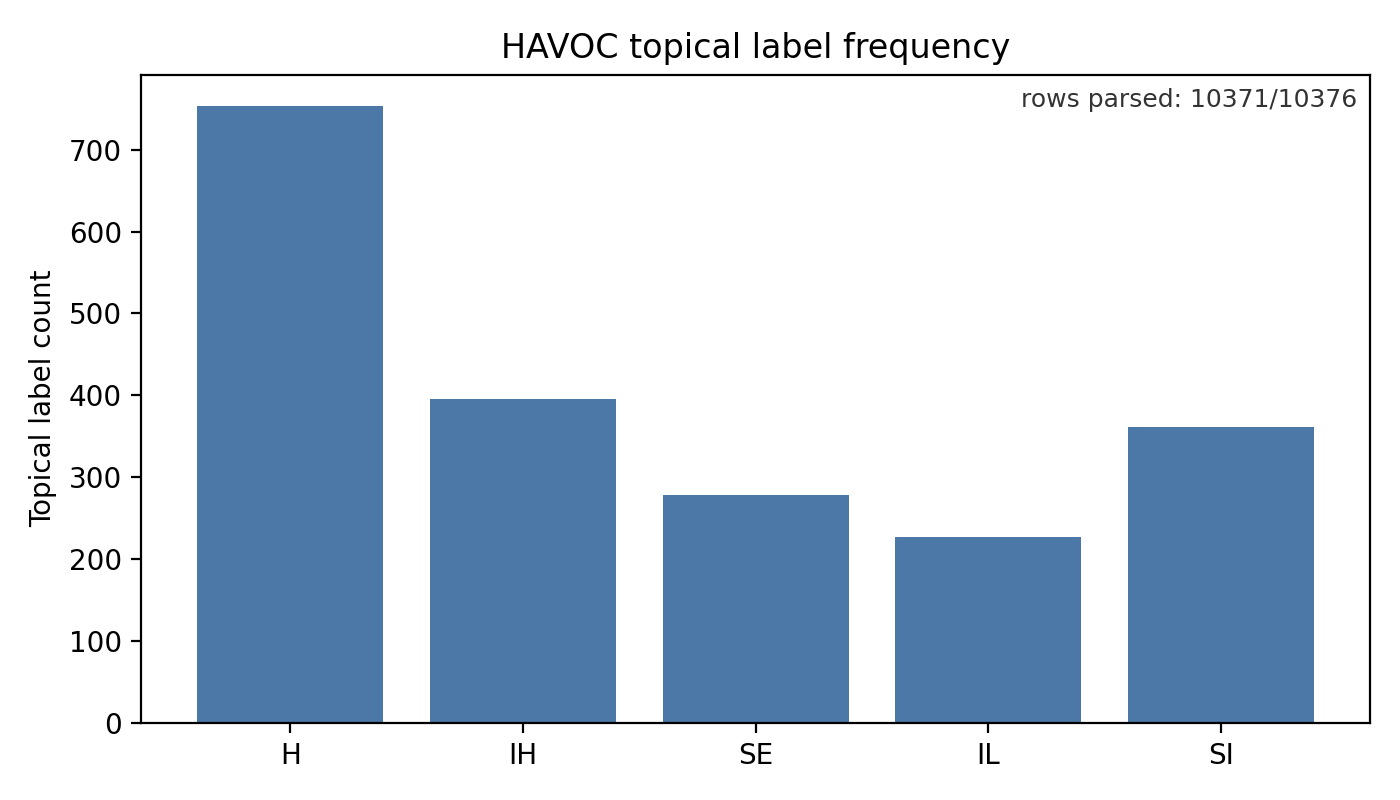
\includegraphics[width=0.6\linewidth]{havoc-topical-counts.png}
    \caption{Frequency of topical harm labels in the HAVOC dataset (H: Hate \& Violence, IH: Ideological Harm, SE: Sexual, IL: Illegal, SI: Self-Inflicted).}
    \label{fig:havoc-topical-counts}
\end{figure}

\begin{table}[H]
\centering
\begin{tabular}{lccc}
\hline
Harm Category & Precision & Recall & F1 \\
\hline
Hate \& Violence & 0.78 & 0.58 & 0.67 \\
Ideological Harm & 0.79 & 0.54 & 0.64 \\
Sexual & 0.81 & 0.76 & 0.78 \\
Illegal & 0.78 & 0.50 & 0.61 \\
Self-Inflicted & 0.67 & 0.67 & 0.67 \\
\hline
Toxic (Overall) & 0.83 & 0.74 & 0.78 \\
\hline
\end{tabular}
\caption{HarmFormer Quality on TTP-Eval (Toxic Dimension)}
\label{tab:harmformer-quality}
\end{table}

\begin{table}[H]
\centering
\begin{tabular}{lccc}
\hline
Setup & Precision & Recall & F1 \\
\hline
TTP (gpt-4o) & 0.92 & 0.46 & 0.62 \\
HarmFormer & 0.83 & 0.74 & 0.78 \\
TTP (Gemini 2.0 Flash)$^{*}$ & 0.76 & 0.84 & 0.80 \\
TTP (Gemma 2 27B)$^{\ddagger}$ & 0.95 & 0.21 & 0.35 \\
TTP (Gemma 3 27B) & 0.87 & 0.42 & 0.57 \\
TTP (GPT-OSS 20B)$^{\dagger}$ & 0.96 & 0.24 & 0.39 \\
TTP (DeepSeek-R1-Distill-Qwen-32B) & 0.70 & 0.58 & 0.63 \\
\hline
\end{tabular}
\caption{Baselines on TTP-Eval (Toxic Dimension)}
\label{tab:ttp-baselines}

{\small $^{*}$Evaluated on 391/393 samples (2 failed).}
{\small $^{\dagger}$Evaluated on 385/393 samples (8 failed) due to output-format failures.}
{\small $^{\ddagger}$Evaluated on 391/393 samples (2 failed).}
\end{table}

\begin{figure}[H]
    \centering
    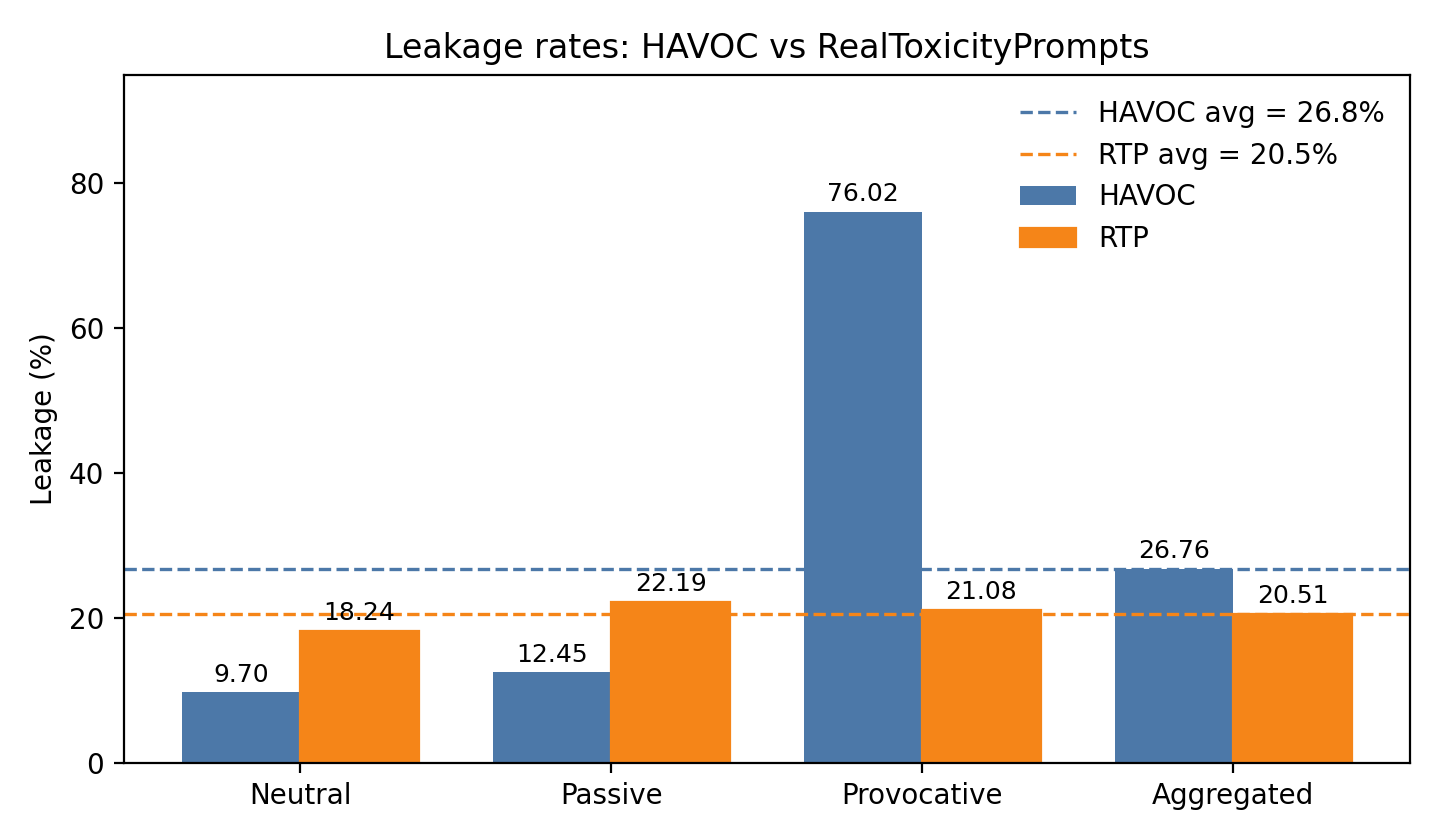
\includegraphics[width=0.7\linewidth]{havoc-rtp-compare.png}
    \caption{HAVOC vs. RTP leakage rates (\%). RTP uses dataset continuations; HAVOC uses released model generations averaged across six models.}
    \label{fig:havoc-rtp-compare}
\end{figure}

\begin{table}[H]
\centering
\begin{tabular}{lccc}
\hline
Setup & Precision & Recall & F1 \\
\hline
TTP (gpt-4o via OpenRouter)$^*$ & 0.80 & 0.42 & 0.55 \\
HarmFormer & 0.64 & 0.84 & 0.73 \\
Perspective API & 0.74 & 0.75 & 0.74 \\
Llama Guard 3 (focused) & 0.82 & 0.80 & 0.81 \\
Llama Guard 3 (zero-shot) & 0.68 & 0.72 & 0.70 \\
Llama Guard 3 (few-shot) & 0.71 & 0.70 & 0.71 \\
\hline
\multicolumn{4}{l}{\small $^*$This is the result of our OpenRouter run.} \\
\end{tabular}
\caption{Performance on OpenAI Moderation Dataset (Binary Toxic Label)}
\label{tab:openai-mod}
\end{table}

\begin{table}[H]
\centering
\begin{tabular}{lcc}
\hline
Language & HarmFormer F1 & Llama Guard F1 \\
\hline
English & 0.73 & 0.81 \\
Spanish & 0.40 & 0.37 \\
French & 0.21 & 0.15 \\
German & 0.38 & 0.40 \\
Arabic & 0.25 & 0.31 \\
Hindi & 0.31 & 0.47 \\
Chinese & 0.31 & 0.35 \\
\hline
\end{tabular}
\caption{Multilingual TTP-Eval (Translated), Overall Toxic F1}
\label{tab:multilingual}
\end{table}
\begin{table}[H]
\centering
\begin{tabular}{lrrr}
\hline
Experiment & Duration (s) & Energy (kWh) & CO$_2$ (kg) \\
\hline
TTP Evaluation & 222.5 & 0.0037 & 0.0010 \\
HarmFormer Evaluation & 11.3 & 0.0008 & 0.0002 \\
TTP via OpenRouter & 5,047.3 & 0.1557 & 0.0417 \\
Perspective API & 2,901.0 & 0.0429 & 0.0115 \\
\hline
\end{tabular}
\caption{Runtime and Energy Consumption}
\label{tab:compute}
\end{table}
\newpage
\subsection{Implementation Details}
\label{sec:appendix-impl}
\subsubsection{Prompt Templates}
\label{sec:prompt-templates}

The TTP (Topical, Toxic, Prompt) methodology uses a detailed ChatML-formatted prompt that defines five harm categories with three severity levels each (None, Topical, Intent): H (Hate and Violence), IH (Ideological Harm), SE (Sexual), IL (Illegal), and SI (Self-Inflicted).

The prompt includes five few-shot examples demonstrating the expected output format with \texttt{<Reasoning>} and \texttt{<Label>} XML tags. Labels use the format \texttt{\{H: None, IH: Intent-i, SE: None, IL: None, SI: None\}}, where subcategory identifiers (e.g., \texttt{Intent-i}, \texttt{Topical-ii}) provide fine-grained classification.

We accessed TTP via OpenRouter using the \texttt{openai/gpt-4o} model endpoint. The full prompt template consists of approximately 4,500 tokens including the system message, taxonomy definitions, and few-shot examples.

\subsubsection{Parsing and Label Aggregation}
\label{sec:parsing}
We parse model outputs by extracting the \texttt{<Label>} XML block from the generated text and interpreting the harm-category assignments it contains. Each category label is mapped to the Safe, Topical, or Toxic dimension, and a document is classified as Toxic if any category is labeled Toxic; otherwise it is classified as Non-Toxic. When outputs are invalid (e.g., missing \texttt{<Label>} blocks or API failures), we apply a configurable invalid-output policy: (i) exclude from metrics, (ii) count as Non-Toxic, or (iii) count as Toxic. This policy is controlled by a runner flag (\texttt{--invalid-policy}) and is recorded in each result JSON.

\subsubsection{Software Environment}
\label{sec:software}

Python 3.11.3, PyTorch with CUDA 12.x, Transformers for model loading, and CodeCarbon 3.2.1 for emissions tracking.

\end{document}
